

\chapter{Preliminaries\label{chap:preliminaries}}

\section{Radioactivity}
Radioactivity is a natural phenomenon in which unstable atomic nuclei undergo spontaneous decay, emitting radiation in the form of particles or electromagnetic waves. 
This process occurs in certain types of atoms, known as radioactive isotopes or radionuclides. 
The radioactive atom aims to achieve a state of stability by dispensing energy in the form of ionizing radiation.
Ionizing radiation refers to any form of radiation with enough energy to remove tightly bound electrons from the orbit of an atom.
Among others, radioactive decay releases three main types of ionizing radiation: alpha, beta and gamma. 

\section{Some properties of ionizing radiation}
\subsection{Health risks}% %%{
Several health risks are associated with ionizing radiation.
While traversing the human body, ionizing radiation can interact with living tissues causing damage or mutations of individual cells.
In the long-term horizon, exposure to ionizing radiation might cause cancer or even genetic disorders.
The severity of health problems depends on the exposure time and dose of absorbed radiation.
High doses of ionizing radiation over a short period can cause acute radiation syndrome (radiation sickness), that is manifested by nausea, vomiting, fatigue or even skin burns. 
High exposure to ionizing radiation also cause several neurological or cardiovascular problems or might lead to death.% %%}

\subsection{Activity}% %%{
``Activity'' is one of the terms used to quantify and describe the properties of radioactive sources and is defined as the number of radioactive decays per second.
The unit of activity is called Becquerel ($\si{\becquerel}$) and belongs to SI\footnote{International System of units} units.
In other words, if a radioactive source has activity one Becquerel, it means that one unstable nucleus decays per second (on average, since the decay is a stochastic process).
The standard definition of activity only measures the rate of decay and does not take into account the type or energy of the radiation involved.
However, for the purpose of this thesis, the term activity is used as the number of gamma photons emitted from the source position in any direction per second.
% %%}

\subsection{Inverse square law}% %%{
The inverse square law is a fundamental principle that applies to diverse physical phenomena, including radiation.
The law describes how the intensity of radiation decreases with increasing distance from the source.
The intensity of radiation is inversely proportional to the square distance from the source:
\begin{equation}
  intensity \approx \frac{1}{distance^2}.
\end{equation}
For example, doubling the distance to the source means that the intensity decreases to $\frac{1}{4}$.
As illustrated in \autoref{fig:islaw}, this principle comes from the fact that the radiation spreads out over a larger area when the observer is further away from the source.
This rapid decrease makes the search for sources of ionizing radiation challenging since it limits the sensing range of the sensors.

  \begin{figure}[!h]
    \centering
      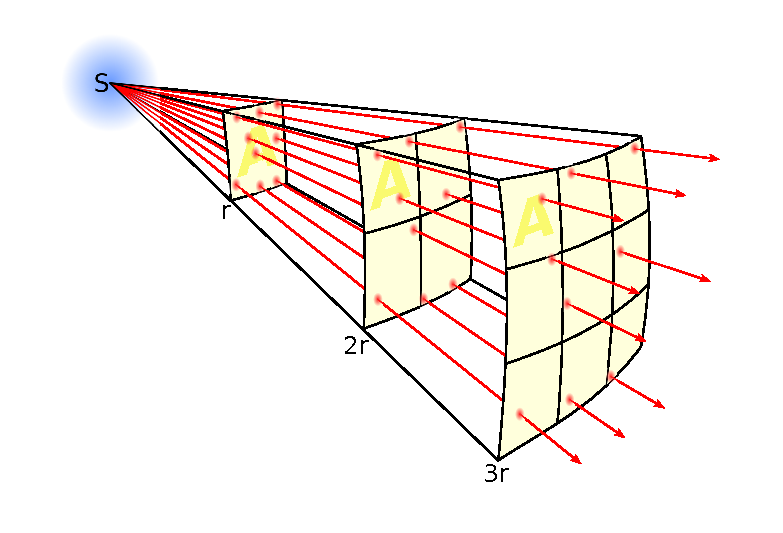
\includegraphics[width=0.65\textwidth]{./fig/photos/Inverse_square_law.eps}
    \caption{An illustration of the inverse square law for the intensity of radiation. Source\protect\footnotemark }%Source: \cite{inverse_square_law}}
      \label{fig:islaw}
  \end{figure}
\footnotetext{\url{https://commons.wikimedia.org/wiki/File:Inverse_square_law.svg}(accessed: 13/05/2023) }
% %%}
\section{Main types of ionizing radiation}
\subsection{Alpha radiation}
Alpha radiation is an emission of positively charged alpha particles consisting of two protons and two neutrons bound together (helium nuclei).
This gives alpha particles a significantly larger mass and higher reactivity compared to other types of ionizing radiation, on the other hand, alpha particles interact strongly with matter and can't penetrate far.
Alpha particles can travel only a few centimetres in the air and can be blocked by a single sheet of paper or the outer layer of human skin.
Because of that, external sources of alpha radiation are generally not considered a significant threat to human health.
The limited range of alpha radiation makes it difficult to sense from a distance.

\subsection{Beta radiation}
Beta particles are high-energy, high-speed electrons or positrons.
Due to their smaller mass and weaker electrical charge, they are generally more penetrating and less reactive than alpha particles and can reach further into materials.
Several centimetres thick sheet of aluminium or plastic is typically sufficient to block weak beta radiation.
In terms of travel through the air, beta particles have a range of a few meters.
Although beta radiation is generally less dangerous than gamma, when particles come into contact with human skin, they can penetrate the outer layers and cause skin burns as the particles disrupt cellular processes.

\subsection{Gamma radiation}
Gamma particles are often produced alongside alpha or beta particles during radioactive decay. 
Unlike the subatomic particles, gamma radiation of composed of high-energy photons. 
$\gamma$ photons are extremely penetrating, can travel long distances in the air and get through most of materials or living tissues thanks to their high energy and lack of charge.
Only a thick layer of concrete or lead might block this type of ionizing radiation.
These features make gamma radiation significantly more dangerous than alpha and beta.
The long-range of gamma radiation, together with its negative effects on human health, motivates the development of methods for the $\gamma$ radiation sensing and detection.
  \begin{figure}[!h]
    \centering
      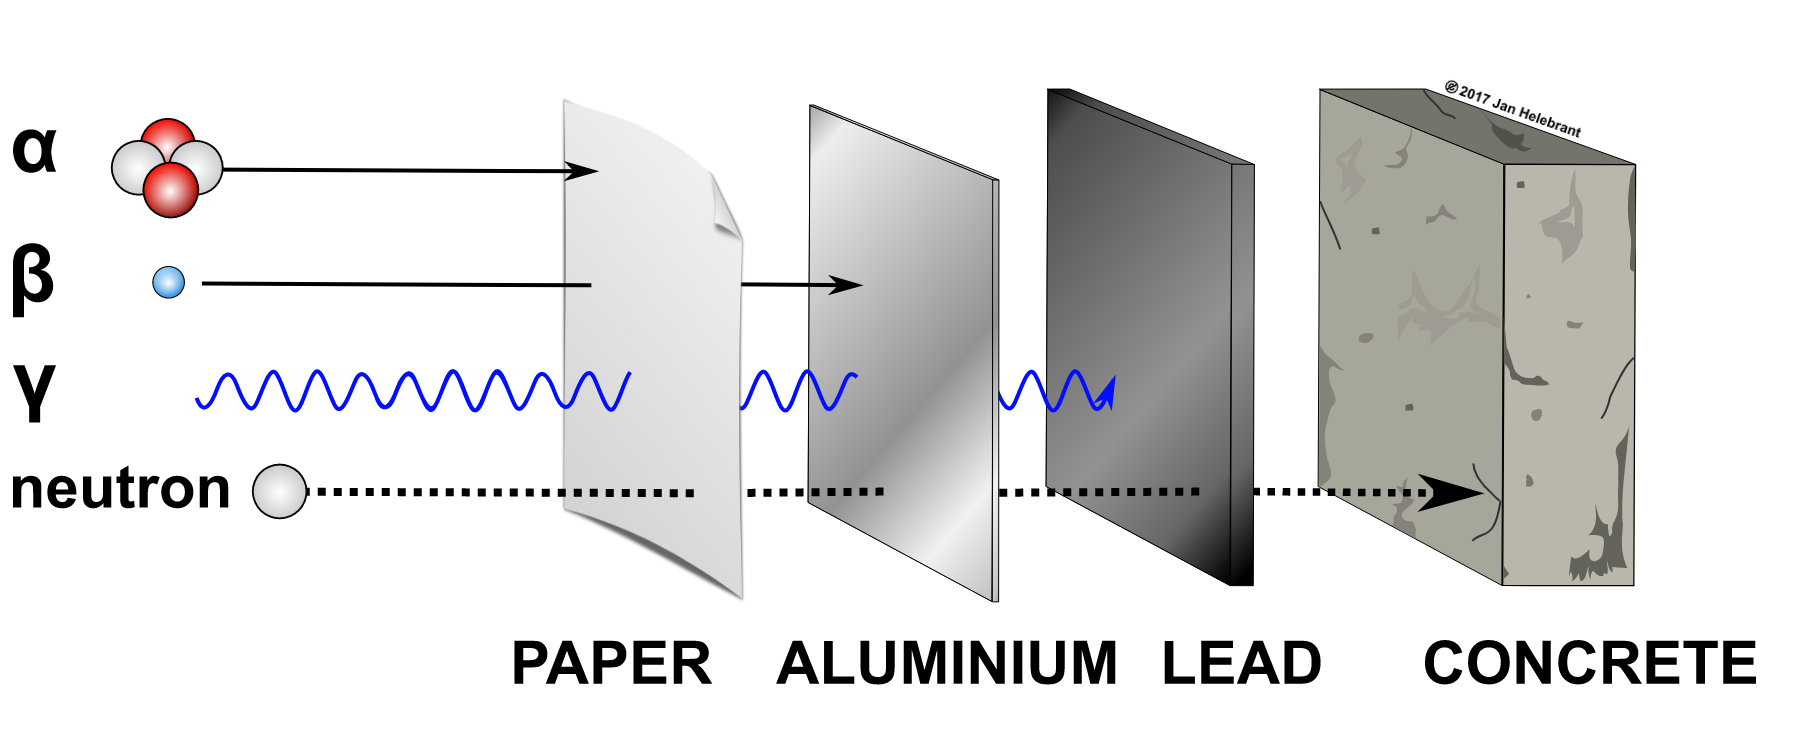
\includegraphics[width=0.6\textwidth]{./fig/photos/pene2.png}
    \caption[x]{Penetrating power of different types of radiation. Source\protect\footnotemark}% \cite{penetrating_power}}
      %\label{fig:islaw}
  \end{figure}

\footnotetext{\url{https://openclipart.org/detail/274074/penetrating-power-of-different-types-of-radiation-alpha-beta-gamma-and-neutrons} (accessed: 08/05/2023)}
\subsection{Cesium-137}
Cesium-137 is a radioactive isotope of Cesium and one of the most common by-products of nuclear fission.
Cesium-137 is used in radiotherapy in medicine, for calibration of radiation detection equipment in the industry and 
(most importantly) it is one of the most common fission products by the nuclear fission of Uranium-235, which is used as a fuel in nuclear power plants and in nuclear weapons.
Cesium-137 is also the main source of radioactive pollution caused by accidents in Chornobyl (1986) and Fukushima (2011).
The half-life (defined as the interval of time required for one-half of the atomic nuclei of a radioactive sample to decay) of Cesium-137 is $30.05$ years.
Notably, Cesium-137 itself is not a source of $\gamma$ radiation.
Cesium-137 decays by beta emission to metastable Barium-137, which decays almost immediately (with a half-life of about $2.5$ minutes) and emits $\gamma$ photons with initial energy $\SI{662}{\kilo\electronvolt}$.
Cesium-137 (with its long half-life, negative health effects, wide usage and high penetrating power of $\SI{662}{\kilo\electronvolt}$ photons) is a good candidate for remote sensing. 
The methods proposed in this thesis have been tested using Cesium-137 radioactive isotope as a source of radiation (during simulated and real-world experiments).

\section{Interaction of $\gamma$ radiation with matter}
Sensing of $\gamma$ radiation is possible through interactions of ionizing photons with imaging devices.
%A variety of interactions may take place as a high-energy photon travels through matter.
Type of the interaction depends on both the energy of the incoming photon and the properties of the material it encounters. 
Several interactions might occur when a high energetic photon travels through matter.
%epending on the energy of the incoming photon as well as on the properties of material.
%Three main types of interactions are: a photoelectric effect, Compton scattering and pair production.
The three primary types of interactions include the photoelectric effect, Compton scattering, and electron-positron pair production.
\autoref{fig:dominant} describes the dominant type of interactions depending on the energy of the incoming photon and the atomic number of the material.

\subsection{Photoelectric effect and pair production}
In \ac{PE}, alternatively referred to as photoelectric absorption, the $\gamma$ photon interacts with an orbital electron of the absorbing atom.
The photon transfers all its energy to the electron and disappears.
As a consequence, the electron exceeds its binning energy and is emitted from the atom.
Photoelectric absorption is dominant at lower energies of the incident photon, although it can occur at any photon energy.
The \ac{PP} occurs only if the $\gamma$ photon has energy exceeding $\approx \SI{1}{\mega\electronvolt}$.
In the pair-production, the highly energetic photon interacts with the atom's nucleus. 
The interaction results in the creation of an electron-positron pair.

\begin{figure}[!h]
  \centering 
    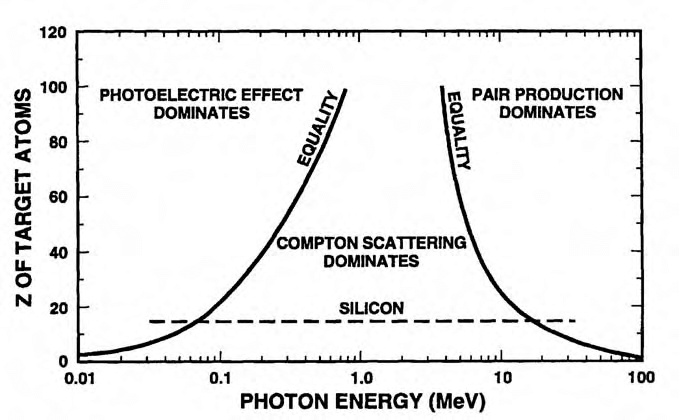
\includegraphics[width=0.6\textwidth]{./fig/photos/dominant.png}
  \caption{Dominant types of interactions for different energy of photon (x-axis) and atomic number of material (y-axis). Source of image: \cite{schwank}}
    \label{fig:dominant}
\end{figure}
\subsection{Compton scattering}
The third potential interaction, primarily prevalent at mid-level energies, is Compton scattering.
In this process, the $\gamma$ photon interacts with an electron that is loosely attached to the nucleus. 
The photon (with its initial energy $E_{0}$) transfers a portion of its energy to the electron.
As a result of the interaction, the lower energetic photon with energy $E_{2}$ is scattered and emitted in a direction changed by angle $\beta$. 
The energy difference $E_{1} = E_{0} - E_{2}$ is transferred to a by-product of the interaction --- an electron.
The situation is illustrated in \autoref{fig:scattering}.
According to Compton \cite{compton}, the relation of particle energies and scattering angle $\beta$ can be expressed as:
\begin{equation}
E_{2} = \frac{E_{0}}{  1 + (E_{0} / m_{e}c^{2}) (1 - \mathrm{cos} \beta)},
  \label{eq:compton_energies}
\end{equation}
where $E_{0}$ is the initial energy of the incoming photon, $E_{2}$ is the energy of scattered photon,  $m_{e}$ is the electron rest mass and $c$ is the speed of light in vacuum. 
\begin{figure}[!h]
    \centering
    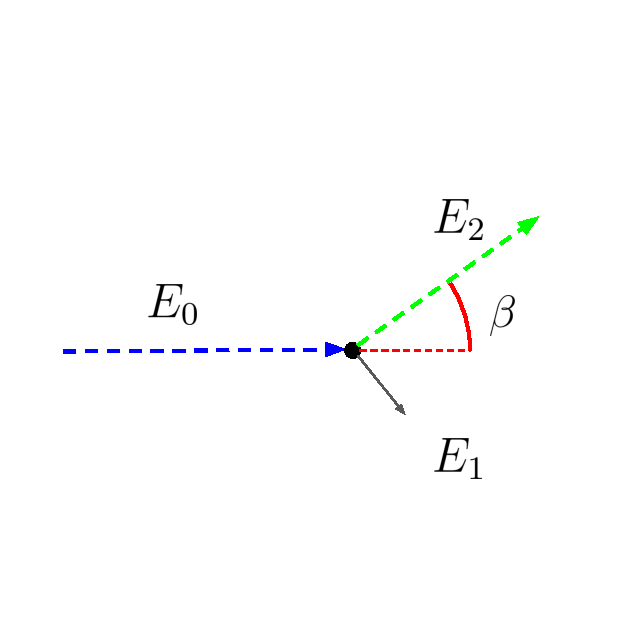
\includegraphics[width=0.4\textwidth]{./fig/photos/compton_simple2.eps}
    \caption{An illustration of the Compton scattering. The incident $\gamma$ photon with energy $E_{0}$ (blue) undergoes the Compton scattering. As a result of the interaction, the lower energetic photon (green) with energy $E_{2}$ is emitted under angle $\beta$. Part of the energy ($E_{1}$) is transferred to a by-product of the interaction---the electron (grey).}
    \label{fig:scattering}
\end{figure}
%%%%%%%%%%%%%%%%%%%%%%%%%%%%%%%%%%%%%%%
\section{Measuring the gamma radiation}
Ionizing radiation is mostly unperceivable by human senses yet poses a significant health risk for human beings. 
Therefore, efficient methods for monitoring and detecting this type of radiation are essential. 
%Various materials that interact with ionizing particles are used to construct sensors for ionizing radiation.
The primary operating mode of most sensors of radioactivity is counting the number of particles detected,
thus estimating the intensity of the particle flux at the sensor's location. 
However, the dosimetric measurements do not provide information about the direction from which the radiation is emitted. 
Intensity-only sensors must be relatively large to get accurate measurements (must collect enough interactions and compensate for the stochastic nature of radioactive decay).
Moreover, the localization of multiple sources might require many measurements at different positions, which is time-consuming. 
The direction of incoming $\gamma$ photons might be deduced using
the Compton camera, which is based on the Compton scattering principle.

\subsection{Compton Camera}% %%{
The Compton camera is typically composed of two detectors: a scatterer and an absorber.
The incident photon with energy $E_{0}$ first interacts with the scatterer at position $X_{1}$ in the form of Compton scattering.
A by-product of the interaction (electron with energy $E_{1}$) is immediately captured by the scatterer, and its position $X_{1}$ and energy are recorded.
As a result of the interaction, a lower energetic photon with energy $E_{2}$ is scattered under (Compton) angle $\beta$.
The scattered photon then interacts in the form of \ac{PE} with the absorber.
The absorbed energy $E_{2}$ and the position of the interaction $X_{2}$ are measured and recorded.

The scattering angle $\beta$ can be reconstructed (following \cite{baca2021gamma}) from equation \autoref{eq:compton_energies} as:
\begin{equation}
  %\beta = \mathrm{arccos} \left (  1-\frac{m_{e}c^{2}E_{2}}{E_{0} (E_{0} - E_{2})} \right )
  \beta = \mathrm{cos}^{-1} 
  \underset{B}{\underbrace{\left (
   1+m_{e}c^{2} \left( \frac{1}{E_{1}+E_{0}} - \frac{1}{E_{0}}\right )  \right )
  }},
    \label{eq:compton_beta_formula}
\end{equation}
assuming that $0<B<1$.
Since Compton scattering is a symmetrical phenomenon,  the set of possible directions of incoming particles forms a surface of a cone.
Such conical surface (denoted as Compton cone) is parametrized by the cone axis $\mathbf{a}$ (which is a straight line connecting the positions of intersections $X_{1}$ and $X_{2}$), Compton scattering angle $\beta$ and origin of the cone $X_{1}$.
The geometry is illustrated in \autoref{fig:compton_camera_geometry}.

\begin{figure}[!h]
  \centering
    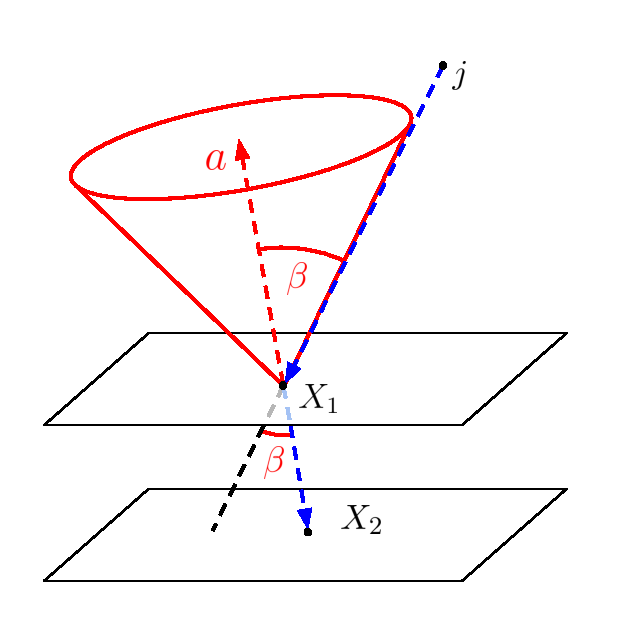
\includegraphics[width=0.4\textwidth]{./fig/photos/compton_camera_modelll.eps}
    \caption{Geometry for two-layer Compton camera. The $\gamma$ particle (emitted at position $j$) interacts with the first layer of the sensor (the scatterer) at position $X_{1}$. A lower energetic photon is scattered under angle $\beta$ and absorbed by the second layer of the detector (absorber) at position $X_{2}$. The reconstructed Compton cone is parametrized by angle $\beta$, axis vector $a$ and origin of the cone $X_{1}$.}
    \label{fig:compton_camera_geometry}
\end{figure}
% %%}

\subsection{The MiniPIX TPX3 sensor} % %%{
The MiniPIX TPX3 detector\footnote{produced by \textit{Advacam}, https://advacam.com/camera/minipix-tpx3} (in the rest of this thesis denoted as \ac{pix} sensor of ionizing radiation) belongs to the class of semiconductor-based radiation sensors.
The \ac{pix} is composed of a) Timepix3 pixel detector \cite{timepix3},
b) the body of the sensor made of a compact block of \ac{CdTe} semiconductor material (with dimensions $14 \times 14 \times 2 \ \si{\milli\meter}$) 
and c) the Minipix readout electronics.
The whole \ac{pix} device is very compact and lightweight (the size of the whole \ac{pix} sensor is only $80 \times 21 \times 14 \ \si{\milli\meter}$ and it weights $\SI{44}{\gram}$), therefore it can be carried onboard a small \ac{UAV}.
Unlike other devices, the \ac{pix} sensor can report the recorded $\gamma$ particles almost in real-time, which allows us to use it for an active strategy, where autonomous \ac{UAV}s react according to the measurements acquired during the flight.

Although \ac{pix} has only one detection layer, it can still be used as a Compton camera.
As described in \cite{baca2021gamma} and \cite{baca2019timepix}, the incoming ionizing radiation interacts with the matter of the sensor and separates electrons from the \ac{CdTe} material.
The separated electrons are accelerated by a $\SI{450}{\volt}$ electric potential towards one facet of the sensor, where the Timepix3 pixel detector is located.
The resolution of pixel detector is $256 \times 256\ \mathrm{px}$, each pixel being $55\ \si{\micro\meter}$ large.
The pixel detector can estimate the energy of the absorbed particle and record the time when it was taken with high resolution.
Given the measured times of arrival, the coinciding products of Compton scattering might be paired together (assuming that both Compton scattering as well as follow-up photon absorption happened at the same time).

\autoref{fig:minipix} depicts the geometry of the \ac{pix} sensor and the detection process.
The x-axis and y-axis coordinates (see \autoref{fig:minipix}) of the interaction are determined by the position of corresponding pixels.
The z-axis coordinate (the depth of interaction in the \ac{CdTe} block) is unknown.
However, the relative z-axis distance of the two coinciding events might be deduced from the times of arrival of the two interactions captured by the pixel detector (given the known speed of electrons in the \ac{CdTe} material).
The absolute z-axis coordinate is not needed since the size of the \ac{CdTe} block is negligible in the context of the detection task.
More technical details related to the sensor operation are provided in \cite{baca2019timepix}.
%The \ac{pix} detector is very compact and lightweight (the size of the whole \ac{pix} sensor is only $80 \times 21 \times 14 \ \si{\milli\meter}$ and it weights $\SI{44}{\gram}$), therefore it can be carried onboard a small \ac{UAV}.
%The \ac{pix} detector can report the recorded intersections almost in real time, which allows us to use it for an active strategy, where autonomous \ac{UAV}s react according to the measurements acquired during the flight.

\begin{figure}[!h]
    \centering
  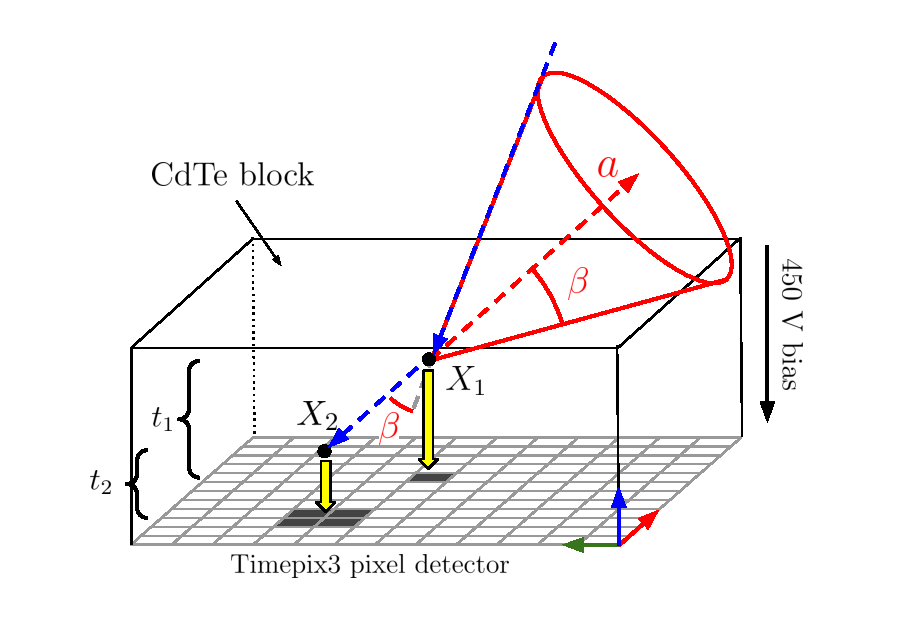
\includegraphics[width=0.7\textwidth]{./fig/photos/my_minipix.eps}
    \caption{An illustration of the detection process inside the \ac{pix} sensor. 
    The incident photon (blue) scatters under angle $\beta$ at position $X_{1}$. 
    %The by-product of the interaction (electron) is immediately absorbed. 
    Scattered photon undergoes photoelectric absorption at position $X_{2}$. 
    The free electrons (produced by the electron's absorption and scattered photon's absorption) are detected by the Timepix3 pixel detector. 2D positions and energies ($E_{1}, E_{2}$) are recorded. 
    The relative z-axis distance between $X_{1}$ and $X_{2}$ is deduced from the time difference $t_{2}-t_{1}$ and the known speed of electrons in the \ac{CdTe} block.
    The Compton cone (red) is then reconstructed.}
    \label{fig:minipix}
\end{figure}

\begin{figure}[!h]% %%{
  \centering
  \subfloat[\centering The real size of \ac{pix} sensor.\newline Source: \cite{baca2021gamma} ] {
    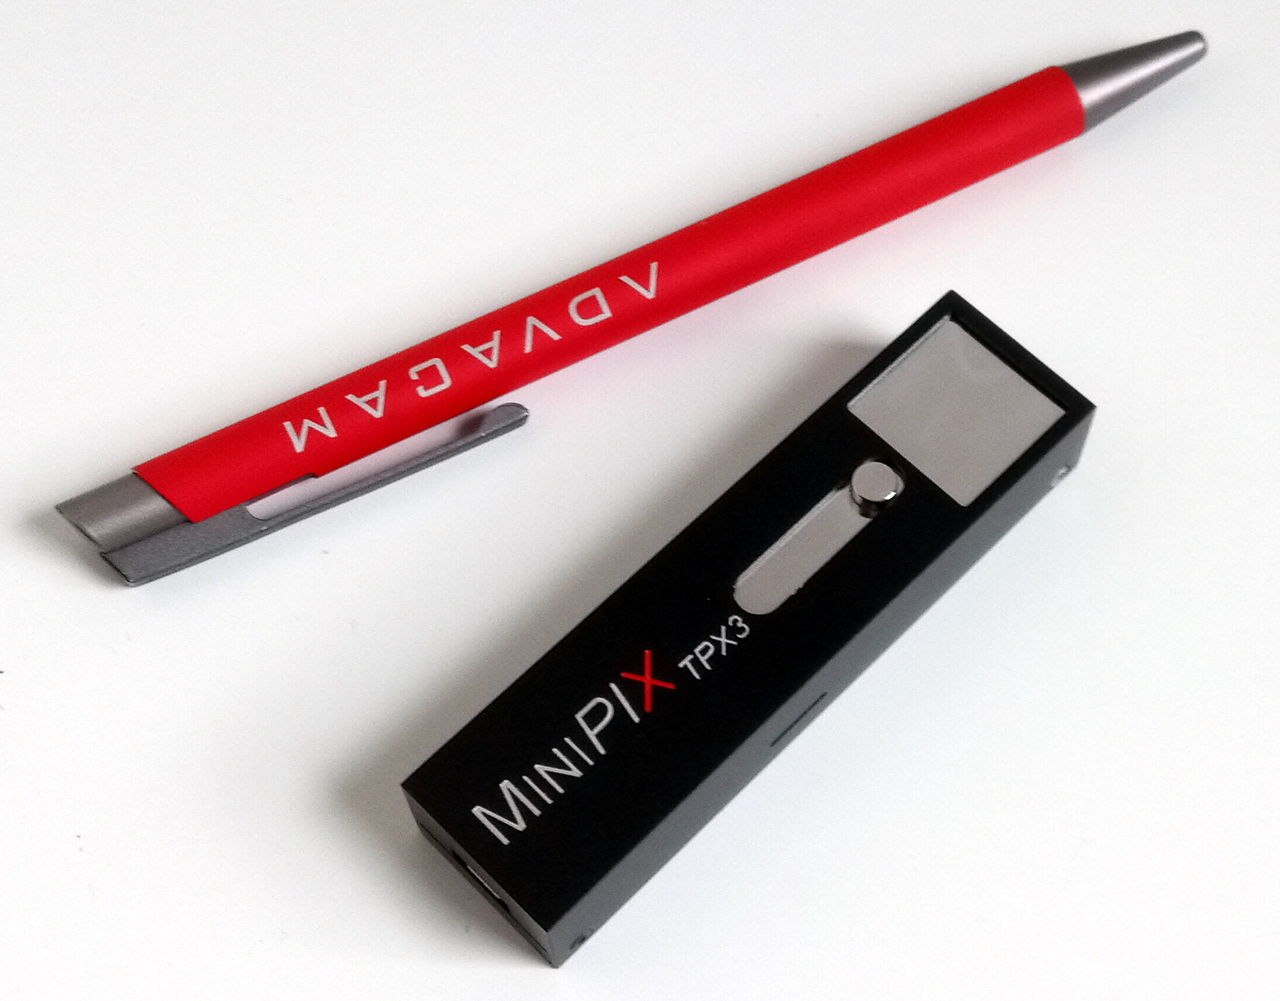
\includegraphics[width=0.4\textwidth]{./fig/photos/minipix_pen.jpg}
    \label{fig:minipix_pen}
  }
  \subfloat[\centering Pixel output of the Timepix3 detector with recorded pair of coinciding events and computed parameters of the Compton cone. Source: \cite{baca2021gamma}] {

    \begin{tikzpicture}
      \node[anchor=south west,inner sep=0] (a) at (0,0) {
          \begin{tabular}{cc}
              \fbox{
\includegraphics[width=0.25\textwidth]{./fig/rviz/timepix_10s.png}}
            &
              \fbox{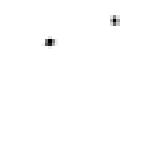
\includegraphics[width=0.25\textwidth]{./fig/rviz/timepix_10s_compton_zoom.png}}
          \end{tabular}
        };

      %%{ labels

      \begin{scope}[x={(a.south east)},y={(a.north west)}]

        \draw (0.37, 0.11) rectangle (0.43, 0.20);
        \draw[black] (0.43, 0.11) -- (0.525, 0.005);
        \draw[black] (0.43, 0.20) -- (0.525, 0.995);

        \draw (0.66,0.80) node [text=black] {\small photon track};
        \draw (0.83,0.95) node [text=black] {\small electron track};

        \draw (0.75,0.36) node [text=black] {
          \begin{tabular}{rl}
            \small $E_{1}$ = &\SI{394.22}{\kilo\electronvolt}\\
            \small $E_{2}$ = &\SI{315.70}{\kilo\electronvolt}\\
            \small $t_{2} - t_{1}$ = &\SI{20.31}{\nano\second}\\
            \small $\Delta z$ = &\SI{0.47}{\milli\meter}\\
            \hline
            \small $\beta$ = &\SI{1.13}{\radian}\\
          \end{tabular}
        };

      \end{scope}

      %%}
    \end{tikzpicture}
  %\caption{An example of a pair of Compton scattering products captured by the Timepix3 detector. The event's times are used together with the particle's energies to reconstruct the scattering angle, $\Theta$.
  \label{fig:timepix_image}





  }
  \label{fig:minipix_ilu}
  \caption{The \ac{pix} sensor and its real size (\autoref{fig:minipix_pen}) and the illustration of output from Timepix3 pixel detector (\autoref{fig:timepix_image}).} 

\end{figure}% %%}

\mycomment{% %%{
\begin{figure}[!h]
    \centering
  \includegraphics[width=0.2\textwidth]{./fig/photos/minipix_in_hand.png}
    \caption{MiniPIX TPX3 sensor. Source: \url{http://mrs.felk.cvut.cz/rospix3}}
    %\label{fig:minipix}
\end{figure}
}% %%}

\mycomment{% %%{
\begin{figure}[!h]
    \centering
    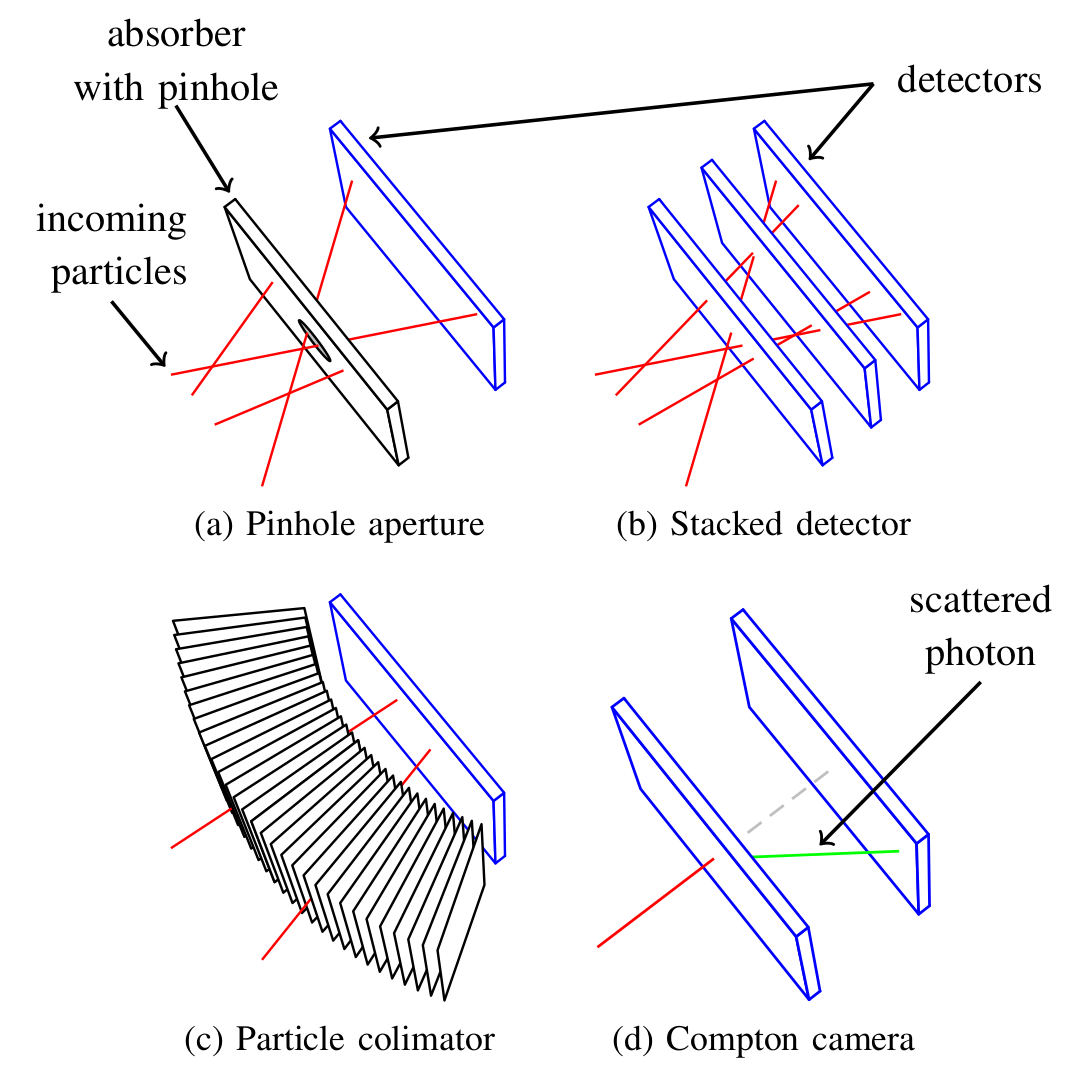
\includegraphics[width=0.5\textwidth]{./fig/photos/detector_overview_baca2019.png}
    \caption{different ways how to detect the direction of incoming particle. Source: \cite{baca2019timepix}}
    \label{fig:sensor_overview}
\end{figure}
}% %%}
% %%}

\section{Robot operating system}
The \ac{ROS} \cite{ROS} is a middleware open-source software framework for robotics applications and research.
\ac{ROS} supports for multiple programming languages, most notably \textit{Python} and \textit{C++}.
Individual software modules (called \textit{nodes}) can exchange data through a standardized communication model.
The registration of the individual \textit{nodes}, as well as communication between them, is maintained by a central authority called \ac{ROS} \textit{master}.
The main advantage of \ac{ROS} is its flexibility --- multiple \textit{nodes} might be executed independently without restarting the whole program.
\ac{ROS} provides a variety of other useful tools.
\textit{TF library} keeps track of multiple coordinate frames over time and provides transformations between them.
\textit{Rosbag} is a tool for recording and playing back data collected during the experiments.
\textit{RViz} is helpful 3D graphical interface for visualisation and debugging.
%The key feature of \ac{ROS} is the \textit{transformation} library, which provides transformations between different coordinate frames of the robotic system.
%The \ac{ROS} master provides the registration of the individual \ac{ROS} nodes as well as maintains communication between them.

\subsection{ROS communication model}
The fundamental \ac{ROS} communication mechanism used for exchanging messages between different \ac{ROS} \textit{nodes} is called \textit{topics}.
\textit{Topics} are based on a publish-subscribe model, where nodes can either publish data to a topic or subscribe to receive data from a topic. 
Each topic has a specific data type associated with it.
Nodes can publish messages of that data type to the topic, and any subscribed nodes will receive those messages.
Topics enable asynchronous communication between different parts of the robotic system, such as data exchange between sensors and onboard computer.

Another important \ac{ROS} communication concept is called \textit{service}.
\ac{ROS} \textit{services} allow \textit{nodes} to make requests and receive responses to them.
Unlike in \ac{ROS} \textit{topics}, services provide a synchronous request-response communication model.
The client node sends its request to a specific service provided by the server node.
The server node processes the request and generates a response message, which is sent back to the sender.
Such a communication scheme might be used, for example, for triggering some action, requesting a path from the planning node and generally in any situation where a response from the server node is required.

\begin{figure}[!h]
    \centering
  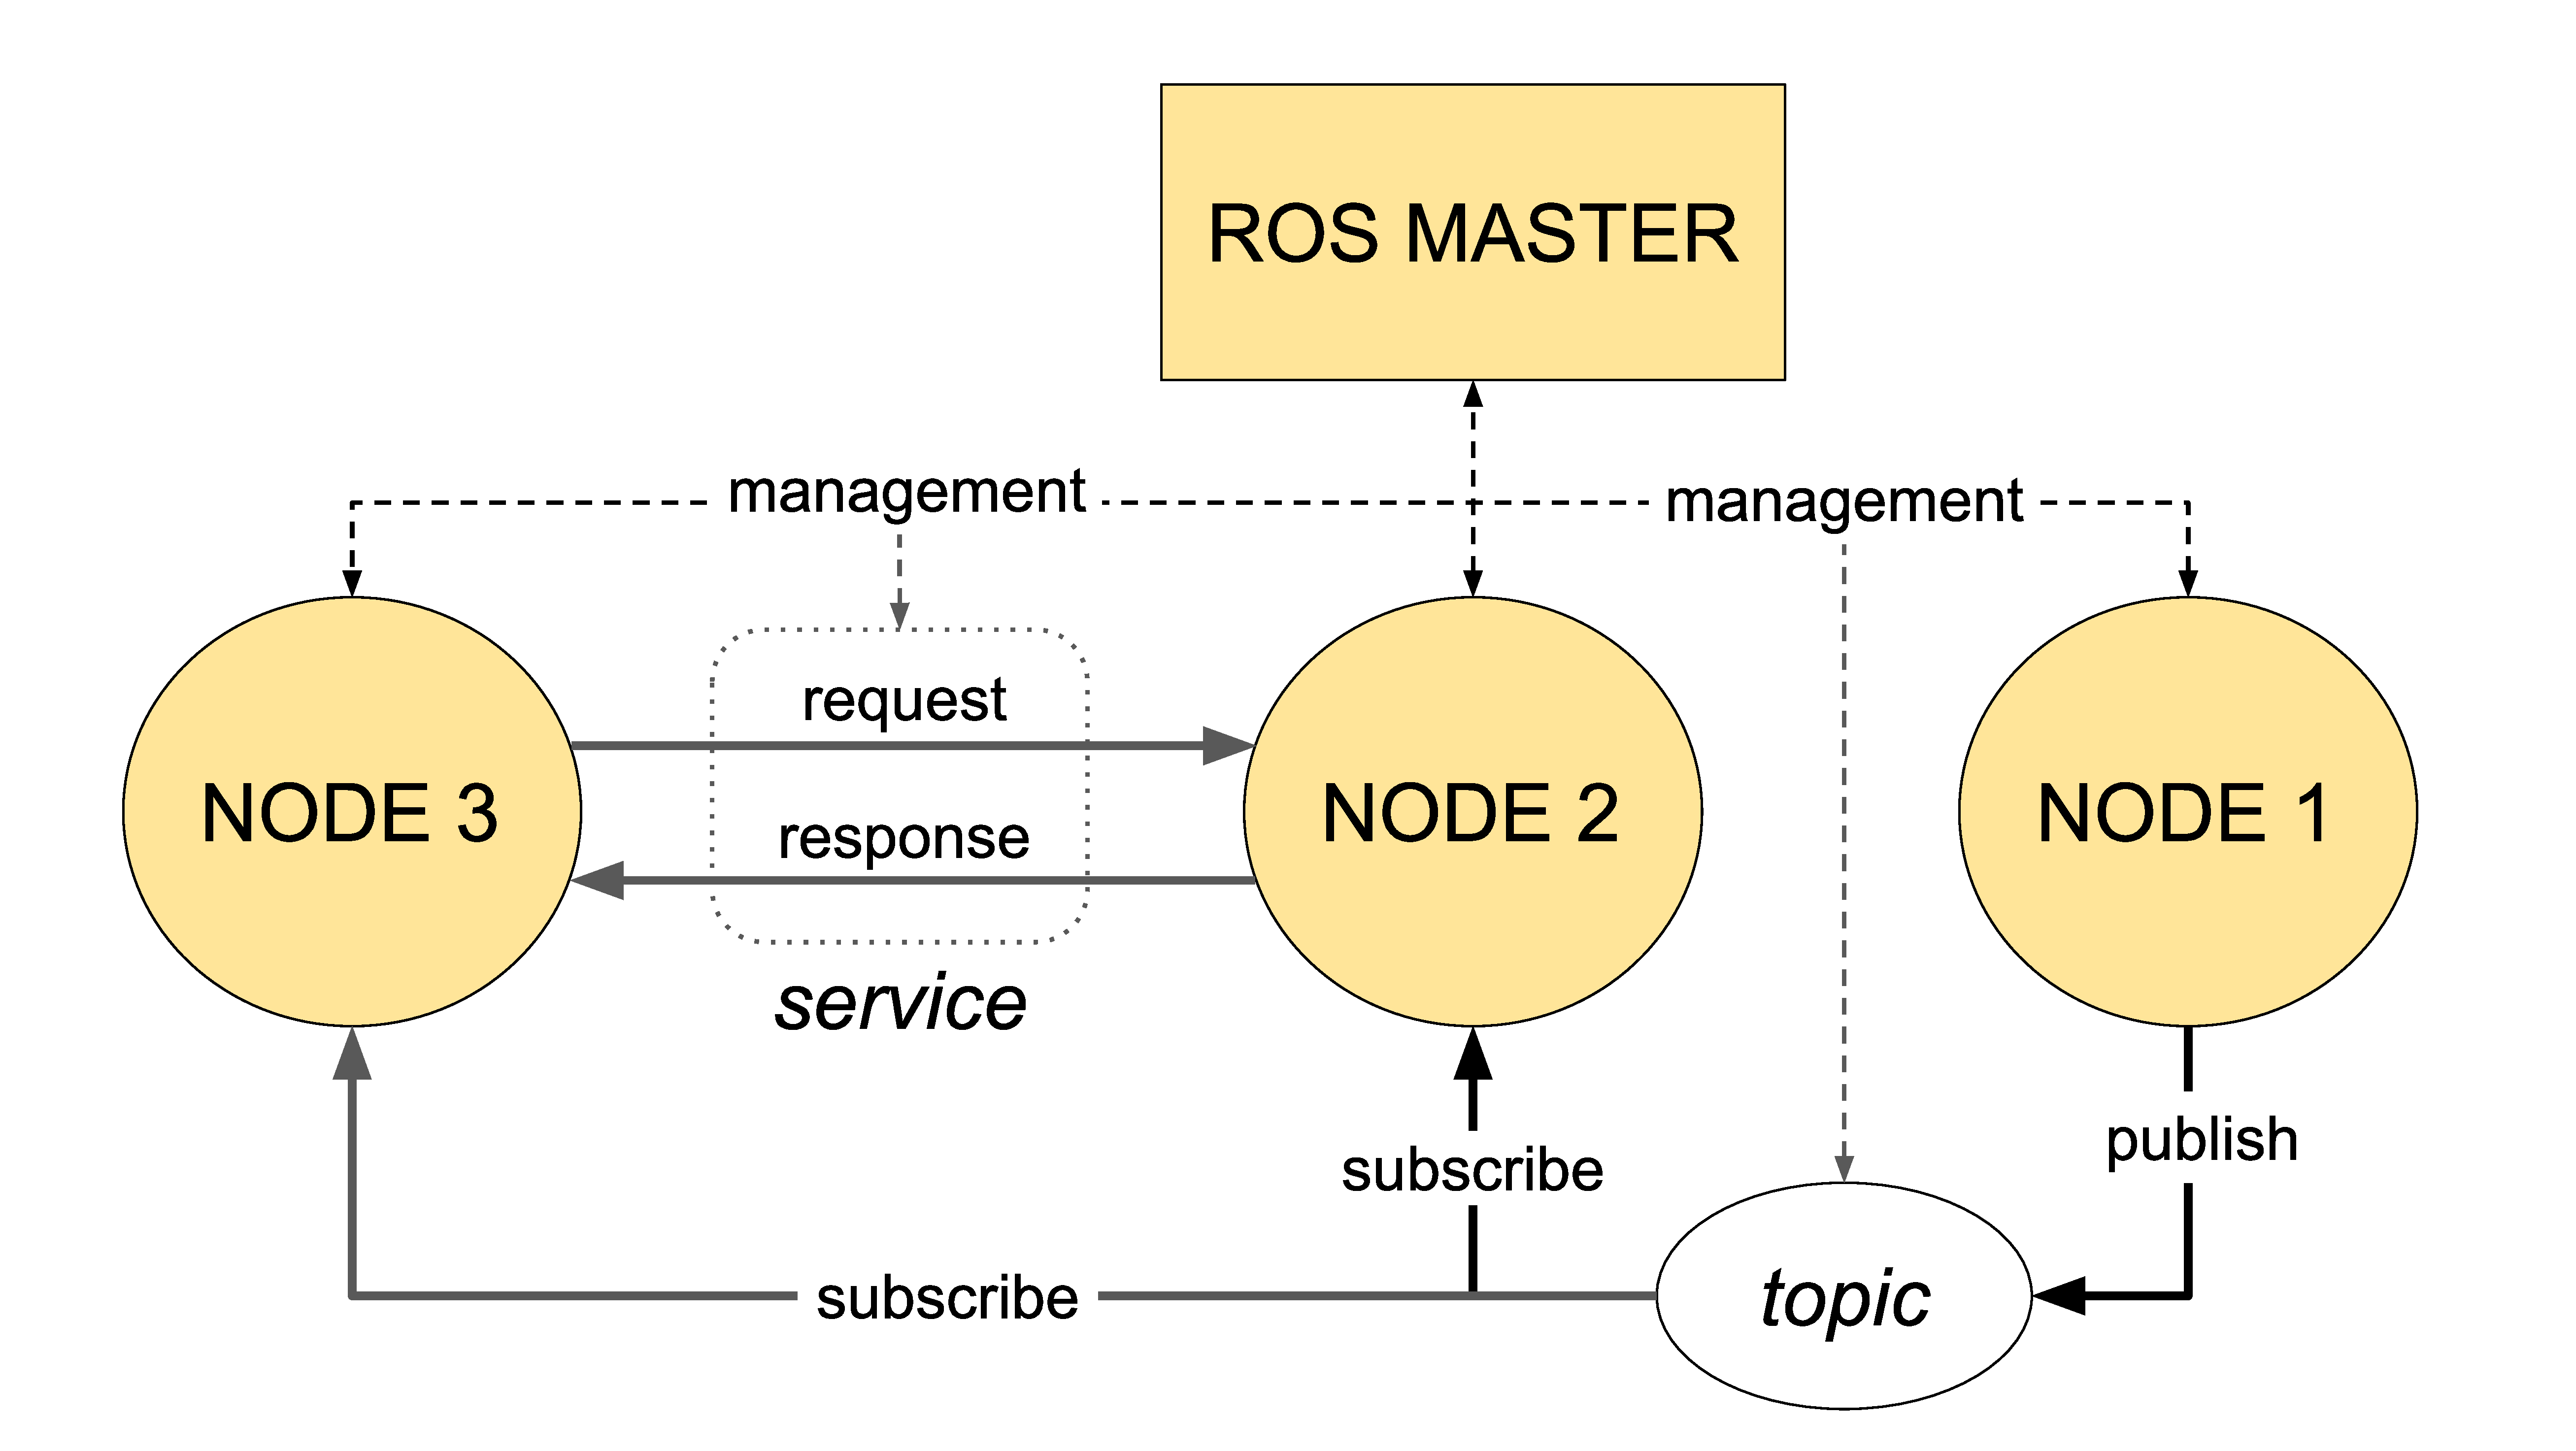
\includegraphics[width=0.8\textwidth]{./fig/photos/ros_schema.eps}
    \caption{Structure of \ac{ROS} communication model. Individual \textit{nodes} share data using \textit{topics} (publisher-subscriber model) or \text{services} (request-response model). The whole communication as well as \textit{node} registration in managed by \textit{master}.}%\url{https://www.clearpathrobotics.com/assets/guides/melodic/ros/Intro%20to%20the%20Robot%20Operating%20System.html}}
    %\label{fig:minipix}
\end{figure}

\subsection{Simulations}
The simulations within this project were made using \textit{Gazebo}, an open-source 3D simulator for robotic research.
Gazebo is fully compatible with \ac{ROS} and allows realistic simulations of robotic systems.
The ionizing radiation was simulated using \textit{Rospix}\footnote{available at: \url{https://github.com/rospix}} simulation package.
The simulation process incorporates properties of the environment (air attenuation) as well as the geometry of the sensor and all the underlying principles leading to the detection of an ionizing photon by the Compton camera.
The properties of the simulator of ionizing radiation are described in \cite{baca2019timepix}.

\section{MRS UAV system}
The proposed high-level search strategy builds on the MRS UAV system\footnote{available at: \url{https://github.com/ctu-mrs/mrs_uav_system}} \cite{mrs_system}.
The MRS UAV system is a research-oriented software platform developed at Czech Technical University in Prague.
The MRS system is based on \ac{ROS} and provides full control pipeline for different types of \ac{UAV}s, including state estimation, sensor fusion, trajectory generation, multi-robot communication, motion planning and feedback control.
%Methods proposed in this thesis builds on some parts of the MRS UAV System --- localization and state estimation (it is assumed the drones are localized using \ac{GPS} or other localization method), communication (the drones can exchange information between each other) and control (the \ac{UAV}s can execute given path).


%%%%%%%%%%%%%%%%%%%%%%%%
%%%%%%%%%%%%%%%%%%%%%%%%%%
%%%%%%%%%%%%%%%%%%%%%%%
%%%%%%%%%%%%%%%%%%%%%%%%%%%%
%%%%%%%%%%%%%%%%%%%%%%%%%%
%%%%%%%%%%%%%%%%%%%%%%%%
%%%%%%%%%%%%%%%%%%%%%%%%%%
%%%%%%%%%%%%%%%%%%%%%%%
%%%%%%%%%%%%%%%%%%%%%%%%%%%%
%%%%%%%%%%%%%%%%%%%%%%%%%%

% %%{
\mycomment{% %%{
Ionizing radiation is unperceivable by human senses yet poses a significant health risk for human beings.
%Sensors of ionizing radiation are made of different materials that interact with ionizing particles.
Therefore, efficient methods for monitoring and detecting this type of radiation are essential. 
Various materials that interact with ionizing particles are used to construct sensors for ionizing radiation.

The basic operation mode of these sensors is counting the number of particles detected, thus estimating the intensity of the particle flux at the sensor's location.
The dosimetric measurements do not provide information about the direction from which direction the radiation is emitted. 
Intensity-only detectors must be relative large to get accurate measurements (must collect enough interactions and compensate the stochastic nature of radioactive decay).  
Moreover, localization of multiple sources might require many measurements at different positions, which is time consuming.
The direction of incoming $\gamma$ photons might be deduced using the Compton camera, which is based on the Compton scattering principle.
}% %%}
\mycomment{% %%{
  %The 
  Geiger-Müller counters, scintillation detectors, and semiconductor detectors (among many others).
   Geiger-Müller counter a tube filled with gas that, when ionized by passing particles, conducts an electrical charge corresponding to the detected particle flux.
  Scintillation contains a luminescent material that emits light when hit by ionizing radiation, 
  which is then transformed into an electrical signal by a photodiode. 
  The third common type of detector is made from semiconductive materials sensitive to ionizing radiation. 
  The ejected electrons from the ionization process can be measured to deduce the type and energy of the incoming radiation.
}% %%}


\mycomment{ %klein nishina % %%{
  The probability that a photon with an energy $E_{0}$ undergoes a Compton scattering through an angle $\beta$ is described by the Klein-Nishina formula
  \begin{equation}
    K(\beta, E_{0}) = \frac{r_{e}^{2}}{2} \left( \frac{E_{2}}{E_{0}}  \right)^{2} \left(  \frac{E_{2}}{E_{0}} + \frac{E_{0}}{E_{2}} - \mathrm{sin}^{2}(\beta)  \right),
    \label{eq:klein_nishina}
  \end{equation}
  where $r_{e}$ is the classical electron radius. 
}% %%}

\mycomment{% %%{
  \section{Measuring radioactivity}
  Ionizing radiation is unperceivable by human senses yet poses a significant health risk for human beings.
  Effective monitoring methods are therefore needed to detect and measure the presence of such radiation. %, that is potentially harmful to human beings.
  %Sensors of ionizing radiation are made of different materials that interact with ionizing particles.
  Therefore, efficient methods for monitoring and detecting this type of radiation are essential. 
  Various materials that interact with ionizing particles are used to construct sensors for ionizing radiation.

  Three common types of these sensors include Geiger-Müller counters, scintillation detectors, and semiconductor detectors (among many others).
   Geiger-Müller counters are tubes filled with gas that, when ionized by passing particles, conduct an electrical charge proportional to the detected particle flux.
  Scintillation detectors work differently. 
  They contain a material that emits light when hit by ionizing radiation, 
  which is then transformed into an electrical signal by a photodiode. 
  The third type of detector is made from semiconductive materials sensitive to ionizing photons. 
  The ejected electrons from the ionization process can be measured to deduce the type and energy of the incoming radiation.

  Most of these sensors function by counting the number of particles detected, thus estimating the intensity of the particle flux at the sensor's location. 
  However, this does not provide information about the direction from which the particles are coming. 
  Following \cite{baca2019timepix}, the direction of incoming particles can be deduced by different detector configurations illustrated in \autoref{fig:sensor_overview}.
  \textbf{Pinhole camera aperture} (which is based on same principles as pinhole camera in classical optics) consists of a small hole in shielding material (e.g. lead), blocking all rays in other directions.
  This approach significantly reduces the field of view of the camera. 
  \textbf{Colimators} (frequently used in medical imaging) also restrict the set of possible directions.
  The openings in the shielding material are organized in a way that each part of the detector is responsible for measuring particles coming from certain direction.
  \textbf{Stacked detectors} employ multiple layers of detectors, where the particle's direction is computed from multiple interactions as the ray passes through the layers.
  Finally, the \textbf{Compton camera} use the Compton scattering for deducing the set of possible directions of the original particle. 



  %Each of the proposed methods have some drawbacks in context of deployment onboard a small \ac{UAV}.
  Intensity-only detectors must be relative large to get accurate measurements (collect enough interactions and compensate the stochastic nature of radioactive decay).  
  Moreover, localization of multiple sources might require many measurements at different positions, which is time consuming.
  The use of collimators or pin-hole apertures is not possible due to their limited field of view and large weight and dimensions (caused by the presence of shielding material, which must be thick enough to effectively block the other rays).
  Multi-stack detectors are complicated 
  \begin{figure}[!h]
      \centering
      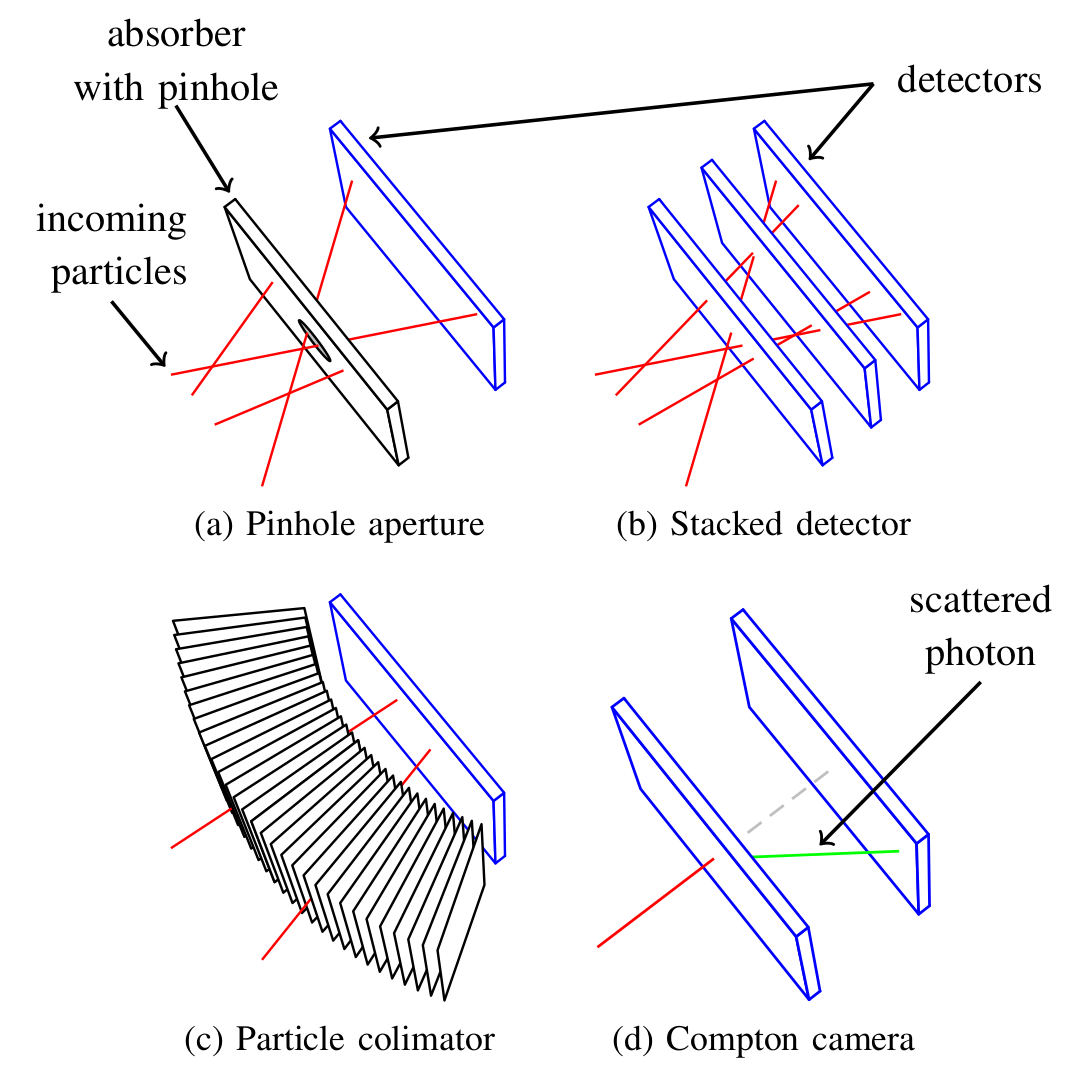
\includegraphics[width=0.5\textwidth]{./fig/photos/detector_overview_baca2019.png}
      \caption{Different ways how to deduce the direction of the incoming particle. Source: \cite{baca2019timepix}}
      \label{fig:sensor_overview}
  \end{figure}
}% %%}

\mycomment{% %%{
\begin{figure}[!h]% %%{
  \centering
  \subfloat[\centering different ways how to detect the direction of incoming particle. Source: \cite{baca2019timepix}] {
    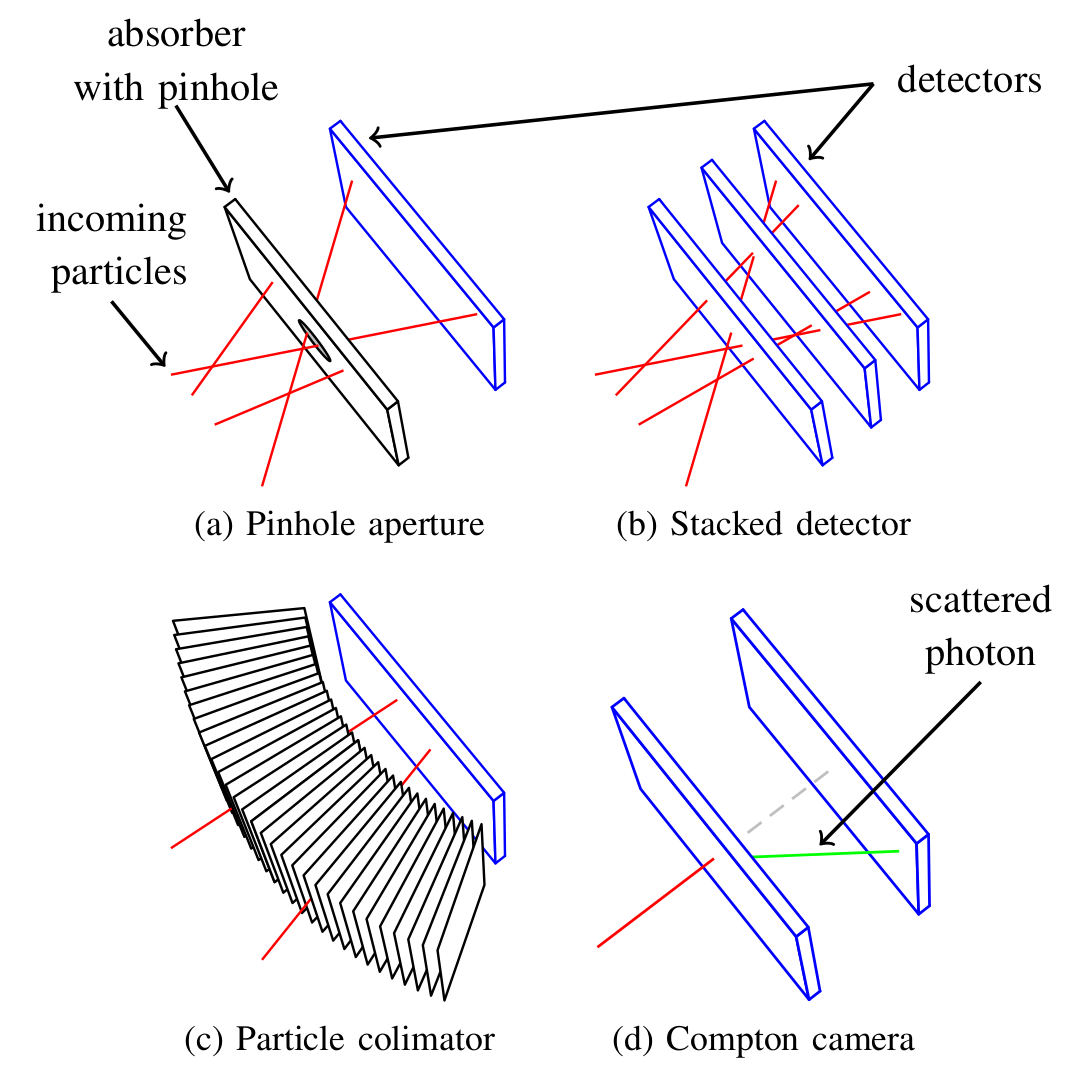
\includegraphics[width=0.49\textwidth]{./fig/photos/detector_overview_baca2019.png}
    \label{fig:sensor_overview}
  }
  \subfloat[\centering Geometry for two-layer Compton camera. The $\gamma$ particle emitted at position $j$ interacts with the first layer of the sensor (scatterer) at position $X_{1}$. A lower energetic photon is scattered under angle $\beta$ and absorbed by the second layer of the detector (absorber) at position $X_{2}$. The reconstructed Compton cone is parametrized by angle $\beta$, axis vector $a$ and origin of the cone $X_{1}$.] {
      \label{fig:compton_camera_geometry}
  
      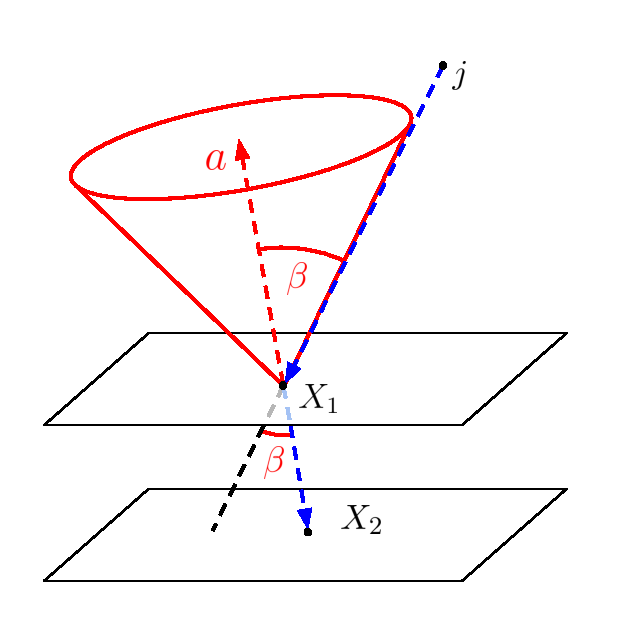
\includegraphics[width=0.49\textwidth]{./fig/photos/compton_camera_modelll.eps}
  }
  \caption{TODO}
  \label{fig:xxx}
\end{figure}% %%}
}% %%}

% %%{
\mycomment{



\begin{figure}[!h]% %%{
  \centering
  \subfloat[\centering Cross-section for photon interactions in Silicon in the MeV range. The four dominating interaction mechanisms are photo effect, Compton scattering, pair creation and Rayleigh scattering. Source: \cite{zoglauer}] {
    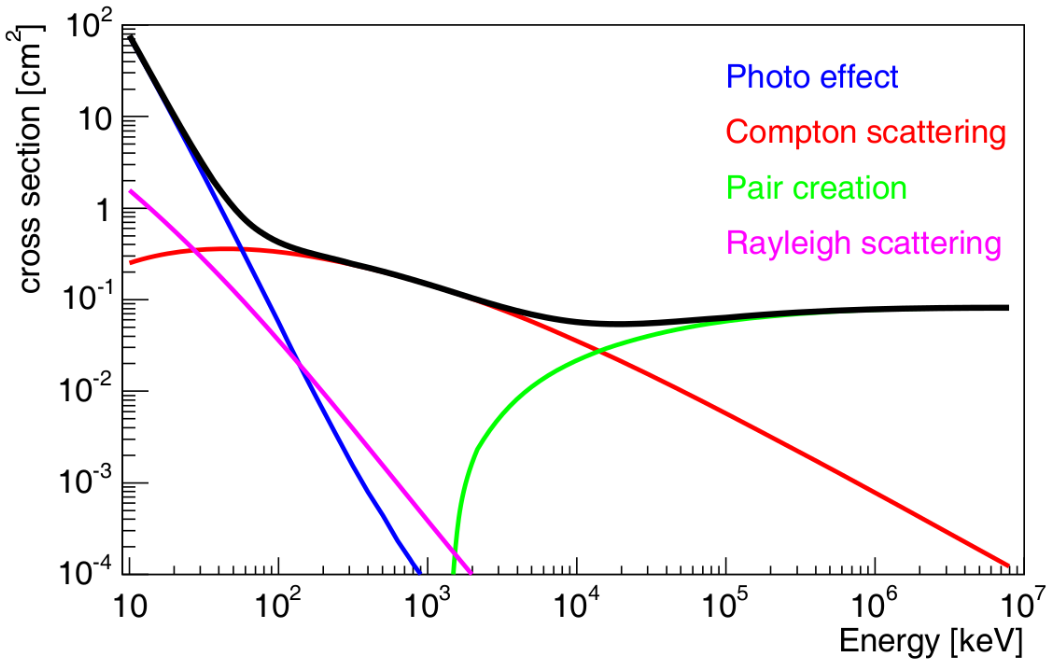
\includegraphics[width=0.2\textwidth]{./fig/photos/cross_stat.png}
    \label{fig:aaaaaa}
  }
  \subfloat[\centering Cross section for compton scattering. Source: \cite{zoglauer}] {

    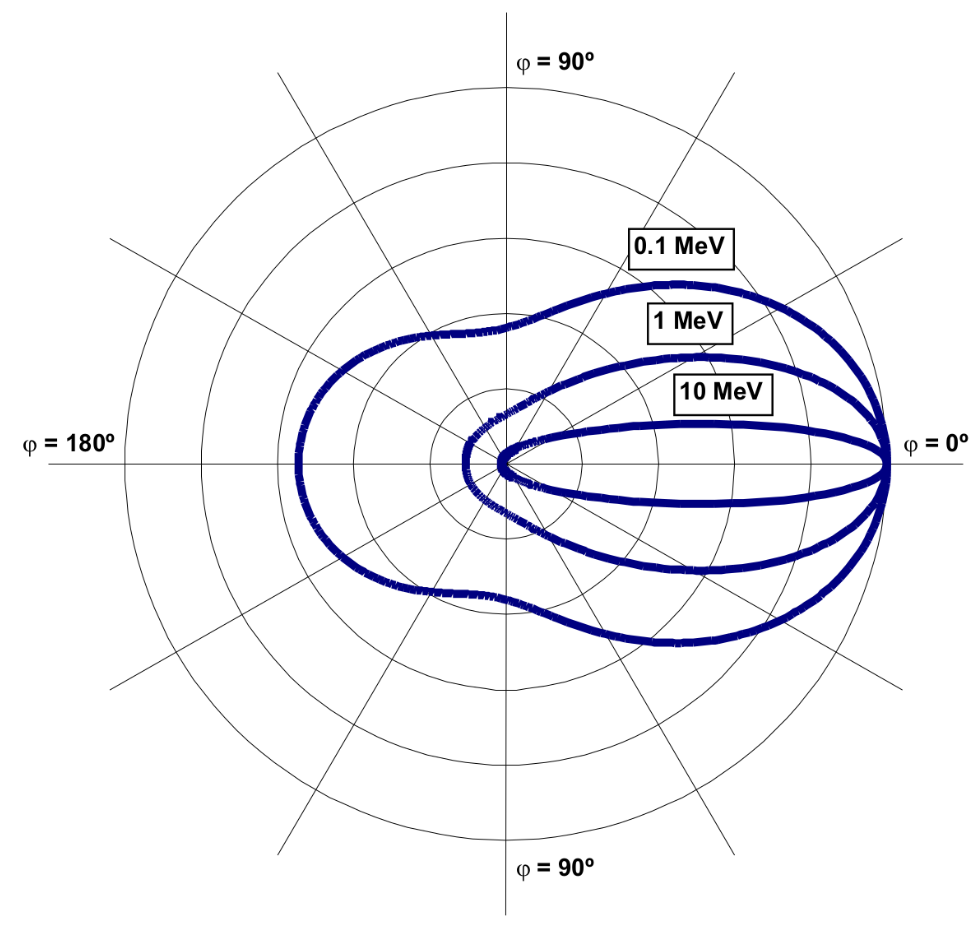
\includegraphics[width=0.2\textwidth]{./fig/photos/cross_section.png}
    \label{fig:aaaaaa}
  }
  \caption{TODO}
  \label{fig:xxx}
\end{figure}% %%}
  \section{Radioactive decay}
  Radioactive decay is a process where an unstable atomic nucleus transforms into a lower-energy state.
  During this process, it loses energy by radiation.
  There are three main types of such radiation - alpha, beta and gamma.
  Whereas alpha particles can be stopped by a sheet of paper and beta particles by aluminium shielding, gamma particles can be blocked only using a thick block of lead or a massive concrete wall.
  Moreover, highly energetic gamma rays have a negative effect on the human body, causing damage on a cellular level.
  Being exposed to such radiation poses a risk of severe health problems or death.

  \section{Some properties of $\gamma$ radiation}
  \subsection{Inverse square law}
  \subsection{Interaction with matter}

  The quantity of emitted particles ("strength" of the source) is expressed in Becquerels.
  It is a SI unit defined as the number of emitted particles per second.

  \section{Interaction with matter}
  As the gamma particle passes through matter, there are three possible effects that might happen:
  \textbf{the photoelectric effect}, \textbf{Compton scattering} and \textbf{pair production}.

  \textbf{The photoelectric effect} is typical at low energies of gamma rays. A photon undergoes an interaction with an electron that is bound in an atom. The incident photon completely disappears in this interaction. A product of this interaction is a photon.
  \textbf{The Compton effect} is typical for mid-energetic gamma rays. In this process, an incident gamma photon loses energy to an atomic electron. A new lower energetic photon is emitted in a different direction (hence the frequently used term "Compton scattering").
  \textbf{Pair production} is typical for high-energetic gamma rays. It is a process in which a photon of sufficient energy is converted into an electron and a positron.

  The Compton effect (published in 1923 \cite{}) describes the way how a (gamma or X-ray) photon interacts with a static electron. An incident photon with wavelength $\lambda$ losses some energy to the electron. A new lower energetic photon with wavelength $\lambda^{\prime}$ is emitted under angle $\beta$. Thanks to the law of conservation of energy and momentum, Compton derived the following equation
  \begin{equation}
      \lambda^{\prime} = \lambda + \frac{h}{m_{e}c}(1-\mathrm{cos} \beta),
  \end{equation}
  where $\lambda$ is the wavelength of the incident photon, $\lambda^{\prime}$ is the wavelength of the emitted photon, $h$ is the Planck constant, $m_{e}$ is the electron rest mass, $c$ is the speed of light and $\beta$ is the scattering angle.

  \begin{figure}[!h]
      \centering
      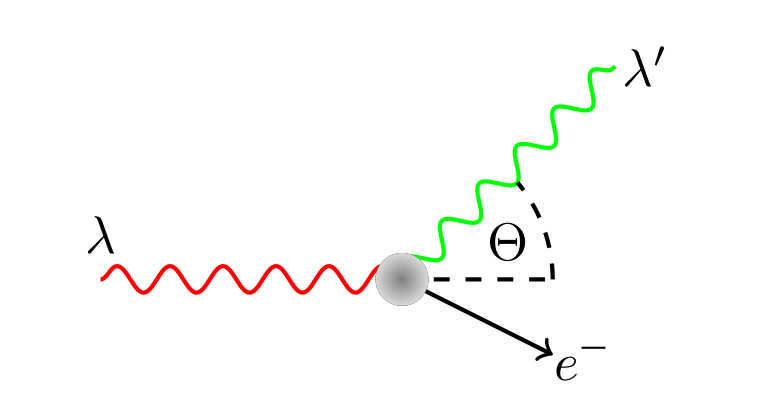
\includegraphics[width=0.3\textwidth]{./fig/photos/scattering.png}
      %\label{fig:scattering}
      %\caption{An illustration of Compton scattering. The incident photon interacts with the static electron. As a result, a new lower energetic photon is emitted in a direction changed by $\beta$ as part of its energy is transferred to electron $e^{-}$. Source: \cite{baca2021gamma}}
  \end{figure}


  \subsection{Klein Nishina formula}
  TODO

  \subsection{Compton effect}
  TODO


  \section{Compton camera}
  This effect is the fundamental principle in a sensor called a Compton camera. 
  The sensor is typically composed of two main components: the scatterer and the absorber. 
  The incident photon first interacts with the scatterer, where the lower energetic photon is emitted under angle $\beta$ (thanks to the Compton effect). 
  Since it is more common to measure energies instead of wavelength, we can rewrite the Compton formula as
  \begin{equation}
  E_{\lambda^{\prime}} = \frac{E_{\lambda}}{  1 + (E_{\lambda} / m_{e}c^{2}) (1 - \mathrm{cos} \beta)},
  \end{equation}
  where $E_{\lambda}$ is the energy of the incoming photon from the source, $E_{\lambda^{\prime}}$ is the energy of the scattered photon.  
  The by-product of the interaction (electron $e_{e^{-}}$) is immediately measured in the scatterer, and its position is recorded.
  Then, the scattered lower energetic photon interacts with the second layer of the sensor - the absorber. 
  The photoelectric effect is witnessed while measuring the product of it - the energy of the electron $e_{\lambda^{prime}}$ and its position on the absorber.

  Now we can express the scattering angle $\beta$ as
  \begin{equation}
      \beta = \mathrm{arccos} \left (  1-\frac{m_{e}c^{2}E_{\lambda^{\prime}}}{E_{\lambda} (E_{\lambda} - E_{\lambda^{\prime}})} \right )
      %\label{eq:compton_beta_formula}
  \end{equation}

  Given the measurements on the scatterer and absorber and computed scattering angle $\beta$ using the equation \autoref{eq:theta} (using known energy of the incoming photon $E_{\lambda}$), we can reconstruct a set of possible directions from where the original photon arrived. Since the Compton effect is symmetrical, the set of possible directions towards the source of ionizing radiation forms a surface of a cone.



  \subsection{MiniPIX TPX3 sensor}
  The sensor used in this work is a small CdTe event-based camera that is capable of witnessing the interactions between gamma photons and the matter of the sensor and reporting them in real time.
  Unlike the traditional model of the Compton camera mentioned before, this is a single-stack detector.
  In other words, there is no distinction between the scatterer and the absorber and all the measurable interactions are happening in one 14x14x2 mm block of CdTe semiconductor material.
  The sensor is capable of measuring a 3D position of the interactions (and distinguishing its type) inside the detector with nanosecond resolution. 
  All these features open the possibility of using it in Compton camera mode.
  Technical details of the sensor are described in \cite{baca2021gamma} and \cite{baca2019timepix}.
  The biggest advantage of this sensor is its small size, low weight and low power consumption.
  Thanks to that, we can use this sensor on board a small UAV. 


  \section{Cs137}

  \section{ROS}

  \section{MRS UAV system}
}
% %%}% %%}


